\chapter{Problem description}
\label{ch:problem}

\section{The existing agent}

The Ms Pac-Man vs Ghosts framework provides the base implementation of the game for this project: to implement an agent, it is required to subclass the abstract generic class {\tt Controller} and implement the {\tt getMove} function.  The method takes one parameter, the game state, which it can query to make a decision on what move to make.  The return type of the method is specified by the generic type parameter of the class instance:  Pac-Man controllers must extend {\tt Controller{$\langle$}MOVE{$\rangle$}} as they need only return a single move for Pac-Man, while ghost controllers extend {\tt Controller{$\langle$}EnumMap{$\langle$}GHOST, MOVE{$\rangle\rangle$}}, as they must return a mapping of ghosts to moves.

The framework calls the {\tt getMove} method every 40~ms; if the method takes longer than that time to run, its return value is discarded and the last move returned by the function is selected.  Thus, the method has a strict requirement on running time.

\citet{Me2012} implemented an agent which used Monte Carlo tree search.  It makes use of a class called {\tt MonteCarloPacManSimulator} (henceforth referred to as the simulator class) which runs simulated games and builds a game tree representation using MCTS.  The agent repeatedly calls on the simulator class to run iterations of MCTS while there is still time remaining.  Once near the deadline, no more simulations are performed: if the agent is at a decision point, i.e., a junction, wall or power pill, the best move found by the MCTS is returned; otherwise, the {\tt NEUTRAL} move is returned, instructing the character to continue in the same direction as before.  The tree is only reset if a move is made, allowing the agent to build on the previous simulations each game tick, increasing the deliberation time.

MCTS works by using simulated ``roll outs'' of game play.  To do this, the simulator class copies the game state and then repeatedly advances it using particular ghost and Pac-Man controllers until some predefined point (e.g. loss of life, change of level, or after a certain amount of time has elapsed).  The agent was written using a highly modular approach, allowing different implementations to be supplied for various aspects, including the ghost controller to use during simulated playouts.  As discussed in chapter \ref{ch:related}, the final score achieved is an order of magnitude better when the ghost controller used during simulations matches the actual opponent.

\section{Proposed additions to the agent}

The idea behind this work is that if the ghost controller used during playouts could somehow learn to better emulate the observed behaviour of the actual opponent during gameplay, it could result in a better final score.  There are various ways that the ghost controller could learn, and these are discussed briefly below.

\begin{figure}
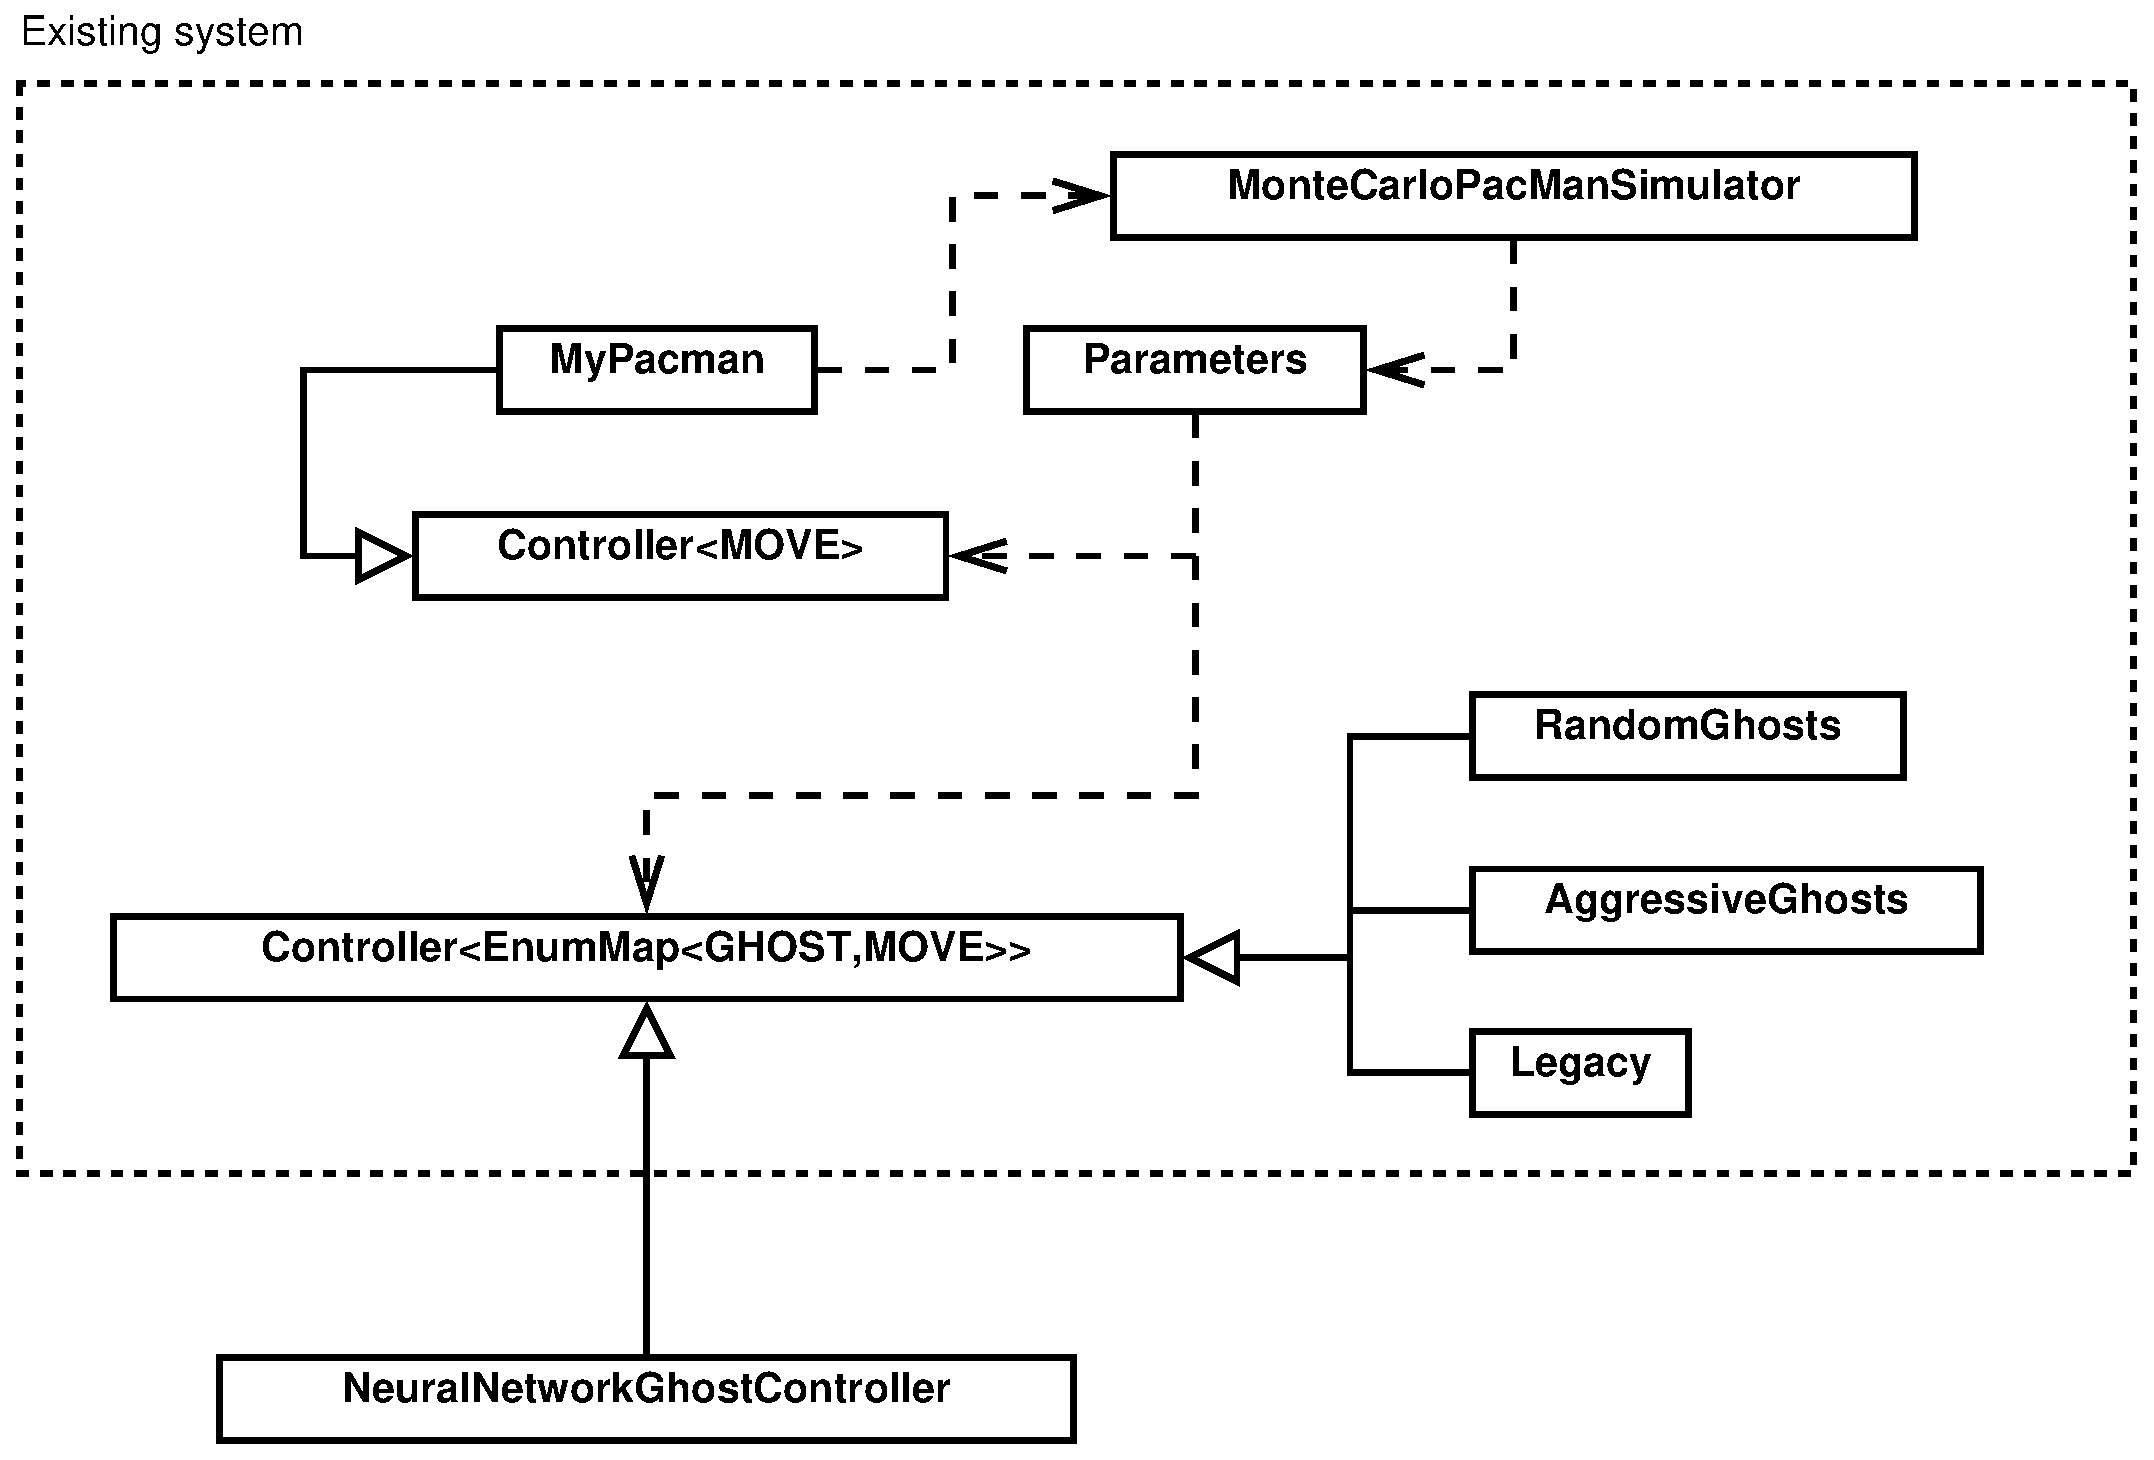
\includegraphics[width=\linewidth]{diagrams/proposed}
\caption[Structural overview]{Structural overview: to implement a Ms Pac-Man agent in the framework, a class extending {\tt Controller<MOVE>} must be created (and it must be called {\tt MyPacman} to be used in the competition).  The existing agent adopts a modular approach: the {\tt Parameters} class contains several fields which specify the behaviour of the algorithm, including one which specifies which ghost controller to use during playouts.  Ghost controllers extend the {\tt Controller<EnumMap<GHOST, MOVE>>} class: some of the example ghost controllers included in the framework are shown.  The proposed addition to the existing agent is a new ghost controller class.}
\label{fig:proposed}
\end{figure}

\subsection{Classifying the ghost behaviour}

One of the first approaches considered at the beginning of this project was to record lots of game data using different opponent ghost controllers, and train a classification algorithm to recognise different kinds of ghost behaviour.  Then during gameplay, the agent could attempt to classify the behaviour observed to determine the known ghost controller which best matches this behaviour, and use this as the controller during playouts.  This has the advantage that a simple classification algorithm, such as logistical regression, is reasonably straightforward to implement.  The downside is that possible opponents in the Ms Pac-Man vs Ghost competitions are extremely diverse, and may not match any of the `known' models.  It would have been interesting to further explore this method if time had available, and it remains a possible opportunity for future work.

\subsection{Reinforcement learning}

\todo[inline]{Reinforcement learning section.}

\subsection{Neural networks}

A neural network is capable of learning behaviour from observed examples, so this seemed like a logical avenue of exploration, and is the method chosen for this project.  Each game tick, the game state is recorded; the following tick, it is possible to retrieve the decisions made on that state for each of the ghosts which needed to make a decision.  This input and observed output is used to train the neural network.

During playouts, the ghost controller uses a neural network for each ghost to decide what moves to return: it feeds as input the elements of game state used during training, and feeds this forward through the network.  Since the network has been trained on the observed behaviour of the opponent, the output of the network should in theory approximate the behaviour of the opponent.

The advantage of this approach is that it should be able to approximate the behaviour of a wide variety of agents.  However, neural network algorithms can be expensive to compute---various optimisations are available but these are often very complex.  Obviously, time spent training the neural network is time that could otherwise be spent on MCTS simulations, so a balance must be maintained.  Furthermore, the agent used during the playouts must feed game state data through the neural networks for each ghost to get predicted moves every simulation tick: this is significantly slower than using a random player and further reduces the amount of simulations that can be run.  A further issue is that a ghost only makes 100-200 decisions in a typical game, and this might not be enough data to train the network particularly quickly.

Finally, at the start of the game before the networks have learnt anything, the ghost controller will effectively be random.  This is not a particularly good choice, and the agent may end up losing all its lives before getting a chance to learn anything.  However, a possible solution to this could be feeding the networks with weights learnt offline on an example controller, so that it is producing at least semi-sensible output even at the start of the game.

\subsection{Requirements}

This discussion draws out a number of requirements.  The addition to the existing agent must perform two functions:

\begin{itemize}
\item Implement a ghost controller which decides on moves player for each ghost, given a game state, using neural networks.
\item Record the decisions of the opponent controller and the game states they were based on each game tick, and use this data to train the neural networks in the ghost controller.
\end{itemize}

Furthermore, the implementation must be fast if it is to be successful.  However, due to the time constraints on the project it may not be possible to implement some of the more advanced algorithms, so a competing requirement is that the implementation must also be reasonably straightforward.

\todo[inline]{Relation to original submitted plan}

\section{Sample ghost controllers}

The Ms~Pac-Man framework used for this project includes several sample ghost controllers.  Although none of them are terribly sophisticated, they provide a basic understanding of the kind of strategies ghost controllers may employ, and are sufficiently different from each other so as to be useful in evaluating the Ms~Pac-Man agent.  They are described briefly below.

\subsection{Legacy}

The {\tt Legacy} controller is designed to be passingly similar to the real ghost AI in Ms~Pac-Man.  For three of the ghosts---namely Blinky, Pinky and Inky---the controller returns the next move which takes the ghost closer to Ms~Pac-Man using the path, Euclidian and Manhattan distance measures respectively.  For Sue, the controller returns a random distance.

\subsection{Legacy2TheReckoning}

The behaviour in this controller is the same for all ghosts:

\begin{itemize}
\item If the ghosts are all in close proximity, but not close to Ms~Pac-Man, they are each sent to their own assigned corner of the maze.
\item If a ghost is edible, or Ms~Pac-Man is close to a power pill, the ghost runs away from Ms~Pac-Man.
\item Otherwise, the ghosts' default behaviour is to chase Ms~Pac-Man.
\end{itemize}

It is more difficult to score points against this ghost controller than the previous as the ghosts retreat when edible, making it more difficult to eat them.  It can be seen that even with just this simple rule, if the {\tt Legacy} controller is used during playouts, but the {\tt Legacy2TheReckoning} controller is the actual opponent, the ghosts will be assumed to be travelling in precisely the opposite direction from their actual direction.

The first rule doesn't change the outcome greatly, as the ghosts are generally only next to each other but not next to Ms~Pac-Man when they are exiting the pen.

\subsection{AggressiveGhosts}

Each ghost is instructed to chase Ms. Pac-Man with a certain probability, or execute a random move otherwise.  The framework version has a hard-coded probability of 1.0, so it was rewritten to allow the probability to be supplied in the constructor.

\subsection{RandomGhosts}

All ghosts play random moves with this controller.  Obviously, any attempt to learn a behaviour from this would not be terribly successful.

\subsection{PansyGhosts}

The ghosts in this controller run away from Ms~Pac-Man with a certain probability, and execute a random move otherwise.  Like the {\tt AggressiveGhosts} controller, the probability has been hard-coded to 1.0 in the framework, so the class was rewritten to accept the probability in its constructor.

\subsection{StarterGhosts}

This controller executes the same behaviour for each ghost:

\begin{itemize}
\item If a ghost is edible, or Ms~Pac-Man is next to a power pill, the ghost runs away from Ms~Pac-Man.
\item Failing that, chase Ms~Pac-Man with a certain probability, hard-coded to 0.9 in the framework.
\item Otherwise, chose a random move.
\end{itemize}

This is fairly similar to the {\tt Legacy2TheReckoning} controller, but with the addition of a random element, and without the dispersal tactic.

